\chapter{Color Coding}

Nel capitolo viene descritta la tecnica del Color Coding utilizzata in questo studio.

La tecnica fu presentata per la prima volta nel 1995 da Alon, Yuster e Zwick \cite{alon1995color}.
In generale, dato un grafo $G = (V,E)$, il problema dell'isomorfismo dei sottografi  di $G$ \`e un problema $NP-completo$.
Il metodo del Color Coding permette di risolvere sottocasi di questo problema in tempo polinomiale.

Dati due grafi, $ G = (V,E) $ e $H = (V_H, E_H)$, i vertici $V$ di $G$, in cui viene cercato un  sottografo isomorfo ad $H$, sono colorati casualmente di $k = |V_H|$ colori. Se $|V_H| = O(\log(V))$, allora tutti i vertici del sottografo di $G$ isomorfo ad $H$, se esiste, sono colorati da colori distinti.   

Il primo algoritmo che loro descrissero, per\`o, si limitava alla ricerca di sottografi indotti in un grafo, senza farne un conteggio del numero delle occorrenze totali.
 
\`E per questo motivo che in questo capitolo si presenta un'estensione dell'algoritmo descritto da Alon \cite{alon1995color}, per effettuare un conteggio delle occorrenze dei Motif all'interno del grafo.
Dati in input un grafo $ G=(V,E) $ e un numero $ k $, per prima cosa il color coding assegna uniformemente e indipendentemente per ogni nodo di $ G $ un'etichetta in $ [k] := \{1,....,k\} $, indicato come un colore.
L'obiettivo \`e quello di conteggiare il numero di alberi colorati non indotti di $ k-nodi $ in $ G $ - chiamati $ treelet $ - i cui colori non sono ripetuti.
Questo viene fatto in maniera efficiente mediante  programmazione dinamica, una tecnica bottom-up che identifica dei sottoproblemi del problema originario, procedendo logicamente dai problemi pi\`u piccoli verso quelli pi\` grandi.




\section{Algoritmo}
\label{section1}

Qui viene descritta l'estensione dell'algoritmo del color coding che pu\`o contare e campionare treelet (non indotti) colorati uniformemnte a caso.
L'algoritmo consiste in una fase di costruzione e una fase di campionamento, in questo studio per\`o non si vede quest'ultima fase, poich\`e non rilevante ai fini di questa tesi, ma si concentra sulla prima fase.
L'algoritmo inizialmente prevede una fase di colorazione, dove per ogni nodo $ v \in V $ di $ G $ \`e assegnato un colore $ c_v $, scelto indipendentemente e uniformemente a caso da $ [k] := \{1,....,k\} $.
L'obiettivo della fase di costruzione \`e quello di creare una tabella con il conteggio delle occorrenze dei treelet che si possono incontrare in $ G $.
Per ogni nodo $ v $ e per ogni albero colorato $ T_C $ con $ k $ nodi, si vuole un conteggio $ c(T_C , v) $ del numero di copie di $ T_C $  in $ G $ che sono radicate in $ v $ (si noti che qui si intendono copie non indotte).
A questo fine per ogni nodo $ v $ si inizializza $ c(T_C , v) = 1 $, dove T \`e il treelet triviale di 1 nodo e $ C = \{c_v\} $.
Successivamente si esegue una programmazione dinamica per il conteggio di treelet di dimensione $ h = 2,...,k $.
Per ogni h a turno, si considera ogni possibile albero radicato T con $ h \le k $ nodi e ogni possibile insieme di colori $ C \subseteq [k] $ con $ |C| = h $.
Poi, $ \forall v \in V$ di $ G $,si calcola come segue il numero $ c(T_C,v) $ di occorrenze dei treelet (non indotti) radicati in $ v $ isomorfi a $ T $ e i cui colori giacciono nell'insieme $ C $. Si divide idealmente $ T $ in due sottoalberi, unici $ T' $ e $ T'' $  radicati rispettivamente nella radice $ r $ di $ T $ e in uno dei figli di $ r $.\\
Perci\`o $ c(T_C,v) $ \`e dato come segue:
\begin{equation}\label{conta}
	c(T_c,v)=\frac{1}{\beta_T}\sum_{u\sim v}\sum_{\substack{{C',C''\subset C}\\{C'\cap C'' =0}}}c(T'_{C'},v)\cdot c(T''_{C''},u)
\end{equation}

dove $ \beta_T $ \`e una costante di normalizzazione che \'e uguale al numero di alberi di $ T $ isomorfi a $ T'' $ radicati in un figlio di $ r $. Per calcolare $ c(T_C,v) $ si passa attraverso tutti gli archi $ u\sim v $ di $ G $, combinando i conteggi di $ u $ e $ v $. La correttezza e la complessit\`a di questa costruzione, non sono trattate qui,ma vengono dimostrate in \cite{alon1995color}.

\begin{algorithm}[H]
	\SetAlgoLined
	\caption{Fase di costruzione}
 	\textbf{input} : Grafo $ G $, dimensione del treelet $ k $ \;	
 				\For{$ v $ in $ G $}{
 				$ c_v = $ viene assegnato un colore preso da [$ k $]\;
 				$ c(T_{c_v} , v) = 1 $\;
 			}	
 			\For{$ h = 2$ to $ k $}{
 				\For{$ v $ in $ G $}{
 					\ForEach{$ T : |T| = h $}{					
 						\( 	c(T_c,v)=\frac{1}{\beta_T}\sum_{u\sim v}\sum_{\substack{{C',C''\subset C}\\{C'\cap C'' =0}}}c(T'_{C'},v)\cdot c(T''_{C''},u) \)	
 					}
 				}
 			}
 			
\end{algorithm}\mbox{}\\

Come si nota, l'algoritmo itera su tutte le coppie di conteggi $ c(T'_{C'},v) $ e $ c(T''_{C''},u) $ per ogni arco $ u\sim v $ e, se $ T'_{C'}, T''_{C''}  $  possono essere unite in un albero colorato $ T_C $, allora si aggiunge $ c(T'_{C'},v) \cdot c(T''_{C''},u)  $ al conteggio $ c(T_C,v) $.
Per fare questo \`e necessaria un'operazione di ``controllo e unione'', che risulta abbastanza costosa.
Infatti, per calcolare $ c(T_C,v) $, per ogni coppia di conteggi 
Una semplice analisi ha restituito il seguente limite di complessit\`a:

\newtheorem{teorema}{Teorema}[section]
\begin{teorema}
	(\cite{bressan2018motif} \textit{Teorema 5.1} ) La fase di costruzione richiede tempo $ O(a^{k}|E|) $ e spazio $ O(a^{k}|V|) $, per un qualche $ a > 0 $.
	
\end{teorema}

La grandezza della tabella ottenuta da questa programmazione \`e il problema maggiore per l'algoritmo, infatti per $ k=6 $ e $ |V| = 5M $, sono necessari $ 45G $ di memoria.

Come si pu\'o notare, per calcolare le occorrenze di un albero $ T $ nell'algoritmo si sfrutta un approccio top-down, ossia a partire dall'albero $ T $ si identificano i due alberi $ T' $ e $ T'' $ in cui pu\`o essere scomposto e in seguito si procede al calcolo di $ c(T_C,v) $ come indicato in \ref{conta}.

In questo studio, invece, si \`e sfruttato un approccio bottom-up. Infatti, per ogni nodo $ v \in V $ di $ G $ e per ogni nodo $ u $  adiacente a $v$, si prendono tutti le coppie possibili di treelet colorati radicati rispettivamente in $ u $ e $ v $, $ T'_{C'} $ e $ T''_{C''} $, entrambi di dimensioni minori di $ h $, con $ h \le k $.
Se $ C' \cap C'' = 0 $ e la struttura di $ T''_{C''} $ \`e minore della struttura del pi\`u piccolo sottoalbero radicato nella radice di $ T'_{C'} $, secondo l'ordinamento totale dei treelet (vedere \ref{section 2}), allora i due treelet possono essere uniti a creare $ T_C $ di dimensione esattamente $ h $ le cui occorrenze saranno determinate come in \ref{conta}.

\section{Struttura dati}
\label{section 2}
In questa sezione vengono descritte le strutture dati usate per implementare l'algoritmo in Java.
Gli oggetti principali che vengono manipolati sono i treelet colorati e le occorrenze associate.

Ogni treelet ha una rappresentazione unica, nella quale sono memorizzati anche i colori.
Vengono codificati come stringhe binarie da 64 bit.
I bit sono cos\'i suddivisi : 
\begin{itemize}
	\item i bit da 0-3 contengono la dimensione del treelet a meno della radice
	\item i bit da 4-7 contengono la dimensione del sottoalbero pi\'u piccolo radicato nella radice del treelet
	\item i bit da 8-11 vengono usati per memorizzare il valore di $ \beta $ associato al treelet.
	\item i bit da 12-27 sono usati per indicare i colori dell'albero
	\item i bit da 28-58 sono usati per codificare la struttura del treelet .
	\item gli ultimi 4 bit sono lasciati a zero
\end{itemize}

		\begin{figure}[htbp]
	\centering
	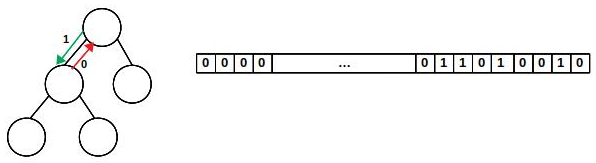
\includegraphics[width=11cm]{capitolo2/grafo3}
	\caption{Un treelet radicato e la codifica della sua struttura}
	\label{figura}
\end{figure}
Per codificare la struttura dell'albero si procede nel seguente modo.
Si esegue una visita DFS trasversale su $ T $ partendo dalla radice $ r $. Poi l'$ i $-esimo bit della codifica \`e 1 (rispettivamente 0) se l'$ i $-esimo arco si visita in direzione opposta a $ r $ (rispettivamente se si visita in direzione di r). In Figura \ref{figura} si pu\`o vedere un esempio di tale codifica.

Per un qualunque $ k \le 16 $ questa codifica richiede al massimo 30 bit.
L'ordinamento lessicografico sulla struttura permette anche un'ordinamento totale sui treelet. Questo ordinamento \`e anche una regola decisiva per la visita DFS: i figli di un nodo vengono visitati nell'ordine dato dai sottoalberi radicati in esso.
Ci\`o implica che ogni treelet $ T $ ha una codifica unica ben definita della struttura. Inoltre, in questo modo si garantisce un'operazione di unione molto rapida.\\

La codifica dei treelet supporta le seguenti operazioni :
\begin{itemize}
	\item $ \textbf{singleton} $ (int color) : permette di inizializzare un treelet di un solo nodo con il rispettivo colore
	\item $ \textbf{merge} $ ($ T' $,$ T'' $) : fa l'unione di due alberi $ T' $ e $ T'' $, se possibile creando un nuovo albero $ T $ che avr\`a come struttura la concatenazione delle strutture di $ T' $ e $ T'' $.
	Come dimensione, a meno della radice, $ T $ avr\`a la somma delle dimensioni di $ T' $ e $ T'' $ pi\'u 1, ossia il nodo radice di $ T'' $.
	I colori di $ T $, sono dati dall'unione dei colori di $ T' $ e $ T'' $.
	In $ T $ come $ \beta $ viene memorizzato il valore corrispondente a quello di $ T' $ e se la struttura del sottoalbero pi\'u piccolo di $ T' $ \`e uguale a quella di $ T'' $ viene incrementato di 1. Per finire, la dimensione del sottoalbero pi\`u piccolo radicato in $ T $ sar\`a esattamente la dimensione di $ T''+1  $ .
	\item $\textbf{normalization\_factor}$ ($ T $): restituisce la costante di normalizzazione $ \beta $.
	    
\end{itemize}
\begin{figure}[htbp]
	\centering
	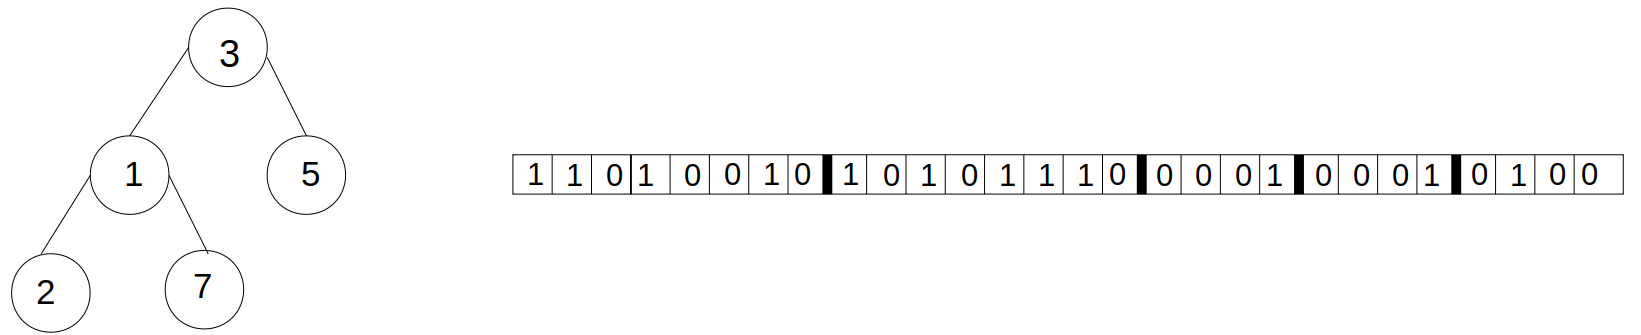
\includegraphics[width=11cm]{capitolo2/grafo4}
	\caption{un treelet colorato e la sua codifica, mostrata per semplicit\`a solo su 8+8+4+4+4=28 bit}
	\label{figura1}
\end{figure}
Un esempio di treelet colorato e della sua codifica \`e data nella Figura \ref{figura1}.



Per quanto riguarda i conteggi delle occorrenze dei treelet sono memorizzati in una tabella con $ k $  entrate ognuna delle quali composta da altrettante $ n $ tabelle, una per ogni nodo $ v \in G $.
La coppia $ (T_C,c(T_C,v)) $ \`e memorizzata in maniera strutturata nelle tabelle, tramite le istanze di una classe $ Entry $, contenente gli elementi della la coppia,  ordinate rispetto la dimensione dei treelet.
Le tabelle sono costruite in maniera dinamica.
La prima tabella, contiene  $ \forall v \in G $ la coppia $ (T_0,1) $ dove $ T_0 $ \`e il treelet triviale colorato.
A seguire sfruttando la variante dell'algoritmo del color coding descritta in \ref{section1} vengono calcolate tutte le tabelle.
Quindi l'$ i$-esima tabella, con $ 2 \le i \le k $, sar\`a costruita sfruttando tutte le $ h-1 $ tabelle gi\`a calcolate.
Cos\`i facendo nella tabella con $ i = k $, saranno contenuti tutti i $ k $-treelet di $ G $ e le loro occorrenze.



	
